\begin{figure}[H]
  \centering

  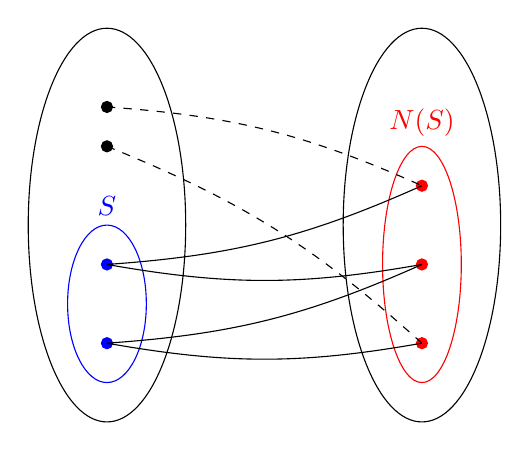
\begin{tikzpicture}
    \coordinate (L1) at (-2, -0.5);
    \coordinate (L2) at (-2, -1.5);

    \coordinate (LS1) at (-2, 1.5);
    \coordinate (LS2) at (-2, 1);

    \coordinate (R1) at (2, 0.5);
    \coordinate (R2) at (2, -0.5);
    \coordinate (R3) at (2, -1.5);

    \draw (-2, 0) ellipse (1cm and 2.5cm);
    \draw (2, 0) ellipse (1cm and 2.5cm);

    \begin{scope}[every path/.style = {color = blue}]
      \draw (-2, -1) ellipse (0.5cm and 1cm);
      \draw node[above] at (-2, 0) {\(S\)};
      \draw[fill = blue] (L1) circle (2pt);
      \draw[fill = blue] (L2) circle (2pt);
    \end{scope}

    \draw[fill = black] (LS1) circle (2pt);
    \draw[fill = black] (LS2) circle (2pt);

    \begin{scope}[every path/.style = {color = red}]
      \draw (2,-0.5) ellipse (0.5cm and 1.5cm);
      \draw node[above] at (2, 1) {\(N(S)\)};
      \draw[fill = red] (R1) circle (2pt);
      \draw[fill = red] (R2) circle (2pt);
      \draw[fill = red] (R3) circle (2pt);
    \end{scope}

    \draw (L1) edge[bend right = 10] (R1);
    \draw (L1) edge[bend right = 10] (R2);
    \draw (L2) edge[bend right = 10] (R2);
    \draw (L2) edge[bend right = 10] (R3);

    \draw[dashed] (LS1) edge[bend left = 10] (R1);
    \draw[dashed] (LS2) edge[bend left = 10] (R3);
  \end{tikzpicture}  
\end{figure}